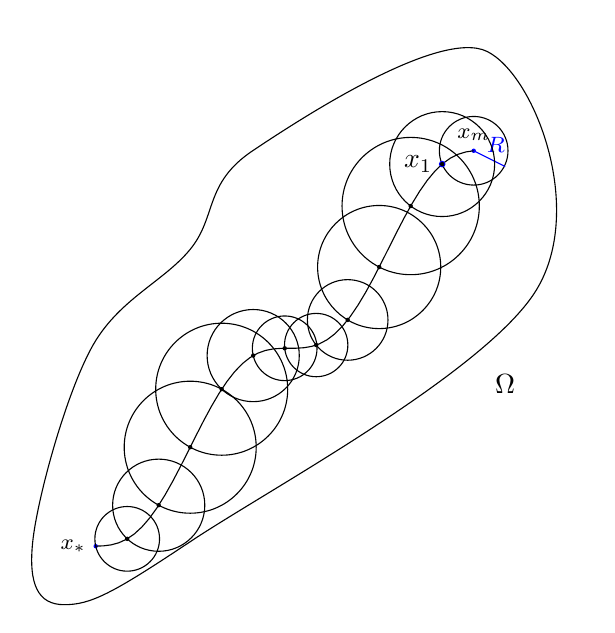
\begin{tikzpicture}[scale=0.4]

% my precious points
\node (xstar) at ({-3 }, { sin(-3 r) - 3 }) {};
\node[left] at (xstar)  {\footnotesize $x_*$ };
\fill[blue] (xstar) circle(2pt);

\node (xm) at ( {9 }, { sin(9 r) + 9 }) {};
\node[above] at (xm) {\footnotesize $x_m$ };
\fill[blue] (xm) circle(2pt);

% initial circle around xm
\draw(xm) circle(31pt);

% draw the radius
\draw[blue, samples=50, -] ( {9 }, { sin(9 r) + 9 }) -- ({9 + 1}, { sin(9 r) + 8.5 }) node[pos=0.7, above] {\footnotesize $R$};

% draw the curve
\draw[samples=50, domain=-3:9] plot ( {\x} , { sin(\x r) + \x} );

% Draw the domain
\draw plot[smooth cycle, tension=0.6]  coordinates { (-pi, pi ) (0, 2*pi) ( 2, 3*pi) (3*pi, 4*pi) (3.5*pi, 5) (0, -3) (-4, -5) (-5, -3) };
\node at (10,2) {$\Omega$};

% mark x1
\coordinate (x1) at (8, {8 + sin(8 r)});
\fill[blue] (x1) circle(3pt);
\node[left] at (x1) {$x_1$};

% draw a bunch of circles
\foreach \p in {8, ..., -2}
{
	\draw ( {\p}, {\p + sin(\p r)} ) circle( { sqrt(1 + (-1 + sin((\p - 1) r) - sin(\p r) )^2  )  }  );
	\fill ( {\p}, {\p + sin(\p r)} ) circle(2pt);
}

\end{tikzpicture}